\documentclass[11pt]{article}
\usepackage[includeheadfoot, top=1.0in, bottom=1.0in, hmargin=1.0in]{geometry}
\usepackage[utf8]{inputenc}
\usepackage{fancyhdr}
\usepackage{url}
\pagestyle{fancy}
\usepackage{setspace}
\usepackage{tabularx}
\usepackage{xcolor}
\usepackage{cancel}
\usepackage{graphicx}
\usepackage{hyperref}
\usepackage{enumitem}
\usepackage{amsmath}
\usepackage[normalem]{ulem}
\usepackage{datetime2}  % customize \today, defaults to yyyy-mm-dd
\lhead{ASTR UN1903 -- AMNH Lab}
\lfoot{M. Sayeed}
\cfoot{\thepage}
\rfoot{\today}
\rhead{Mondays 6-9 pm}
\renewcommand{\rightmark}{}
\renewcommand{\headrulewidth}{0pt}
\renewcommand{\footrulewidth}{0.4pt}

\begin{document}

\begin{center}
\huge{Optional Lab: Eclipses, Upcoming Lunar Eclipse}\\ \medskip \Large{Finish by Nov 27, 2022}
\end{center}

\section{Lab Layout}
This take-home lab is meant to act as extra credit or as a make up for any absences from the in-person labs. It therefore will rely on some independent research, and will include a writing/essay-style questions. Feel free to follow the included links, or to look elsewhere online- but, make sure that all writing is your own original work. Don't copy in any text without proper attribution.

In theory, the links I've provided have all of the information necessary to answer each of these questions, and you're allowed to look elsewhere on the internet as well. So, if you're stuck, the first step is to do some independent research or work together to track down an explanation. 

\section{Eclipse geometry}

\begin{figure}[!h]
    \centering
    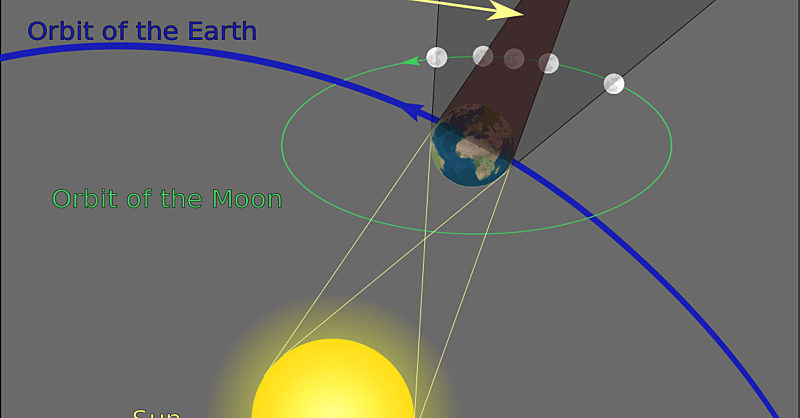
\includegraphics[width=0.7\textwidth]{eclipse_geo.jpg}
    \caption{An illustration of the layout of the sun, Earth, and moon during a lunar eclipse. Credit: The Planetary Society.}
    \label{fig:geometry}
\end{figure}

Eclipses refer to times when three bodies in space all fall on the same line - the exoplanet transits we considered a few weeks ago can be classified as eclipses, since during transit the planet-star-Earth all fall on the same line. Within our solar system, eclipses fall into two flavors: lunar eclipses, when the Earth falls between the moon and the sun, and much more dramatic solar eclipses, when the moon falls between the Earth and the sun. For lunar eclipses, check out the the \href{https://en.wikipedia.org/wiki/Lunar_eclipse}{wikipedia page} or \href{https://moon.nasa.gov/news/185/what-you-need-to-know-about-the-lunar-eclipse/}{this NASA page} about the upcoming eclipse. For solar eclipses, check out \href{https://en.wikipedia.org/wiki/Solar_eclipse}{this wikipedia page} and \href{https://eclipse2017.nasa.gov/eclipse-101}{this NASA page} which was put together ahead of the last solar eclipse visible in the US, in 2017.


With information from those pages, the links within (the Solar Eclipse 101 page is very useful) or other websites, answer the following:
\begin{enumerate}
    \item During what moon phase are lunar eclipses possible, new or full moons?
    \item During what moon phase are solar eclipses possible, new or full moons?
    \item Why don't we see a lunar and solar eclipse every month?
\end{enumerate}


\noindent With the basics of eclipse geometry covered, let's visually combine those answers. Create diagrams of the following situations:
\begin{enumerate}
    \setcounter{enumi}{3}
    \item A top-down view of the sun, moon, and earth during a lunar eclipse happening on the autumnal equinox. Include the locations of each body, circles marking the paths of their orbits, and labels for the autumnal equinox, vernal equinox, summer solstice, and winter solstice. The convention of top-down views of the Earth's orbit is to place the vernal equinox along the positive X axis and assume the Earth moves counterclockwise. 
    \item A top-down view of the sun, moon, and earth during a solar eclipse happening on the summer solstice. Include all the same labels as before.
\end{enumerate}

\section{Lunar Eclipse Colors}
Solar eclipses are dramatic, beautiful events where the sun seems to disappear in the middle of the day. Lunar eclipses are more subtle, but still very strange: the moon doesn't disappear, it just gets darker, then turns a dark red. Using information from online/the same links above:
\begin{enumerate}
    \setcounter{enumi}{5}
    \item Explain why the moon turns red, not some other color.
    \item If the Earth didn't have an atmosphere, what would the moon look like during a lunar eclipse?
\end{enumerate}

% \section{Option 1: Go see the eclipse!}
% Try to see the upcoming eclipse! First, \href{https://www.timeanddate.com/eclipse/lunar/2022-november-8}{check what time the eclipse happens near you}, since that will depend on your location, and some of you may have traveled during the long weekend. Then, using a night sky app, pre-scout your viewing location before it happens to make sure you can actually get to a place where it's possible to see (in most of these apps, you can ``fast forward" time to project the location of the moon at the time of totality). On the night of the eclipse, take and attach a picture of the moon in totality if you're successful. If it's cloudy, attach a picture of the sky/horizon timestamped to show in that in theory you could have seen it- if you went through the effort of setting everything up but were thwarted by something beyond your control, full credit for trying.

\section{Make a hypothetical plan to view the next solar eclipse}
On Monday, April 8th, 2024, a total solar eclipse will be visible along a narrow corridor running across the United States. Using information from \href{https://solarsystem.nasa.gov/eclipses/2024/apr-8-total/overview/}{NASA},  \href{https://www.greatamericaneclipse.com/future}{Great American Eclipse}, or elsewhere, write a $\sim$500 word hypothetical plan to view the eclipse. Be sure to include:
\begin{itemize}
    \item Where you would go. When deciding, consider the visibility of the eclipse from your location, the feasibility of getting there, how cloudy it is in April historically (it'd be awful to make a trip far away and hit clouds), and if there's any other draws to the area besides the eclipse.
    \item A timeline of what you would see in the sky- when would you notice something weird was happening with the naked eye? When would you notice something was weird if using eclipse glasses?    \item What you would see during the eclipse: what is the outermost edge of the sun called? What does it look like? What about the stars?
    \item Any equipment you would need to observe the sun.
    \item This isn't strictly part of a plan, is fun to imagine: if you were standing on the moon looking up at the Earth during this event, what would you see? Why?
\end{itemize}


\section{Conclusions}
\noindent Please complete this section on your own.
\begin{enumerate}

\item What was your favorite and least favorite parts of this lab?

\item What is a question you still have at the end of this lab?

\end{enumerate}

\end{document}